\documentclass[11pt]{article}

\usepackage[margin=1in]{geometry}
\usepackage{amsmath,amssymb,amsthm}
\usepackage{booktabs}
\usepackage{graphicx}
\usepackage{hyperref}
\usepackage[numbers,sort&compress]{natbib}
\usepackage{xcolor}

\newcommand{\todo}[1]{\textcolor{red}{\textbf{[TODO: #1]}}}
\newcommand{\methodloits}{\textsc{LOITS}}
\newcommand{\methodnf}{\textsc{NF}}

\title{MCMC-Corrected Local Inverse Transform and Normalizing-Flow Proposals for Inverse Inference}
\author{
  Jitao \todo{family name} \and Yaohang Li
  \\
  \todo{Department, institution, city, country}\\
  \texttt{\todo{corresponding author email}}
}
\date{\today}

\begin{document}
\maketitle

\begin{abstract}
Inverse inference workflows frequently map samples through inverse cumulative distribution functions or Markov chain Monte Carlo (MCMC) transitions. These operations can be useful for event generation but can obstruct direct gradient propagation. We study two proposal mechanisms followed by a Metropolis--Hastings correction: local inverse transform sampling (\methodloits) and normalizing-flow (\methodnf) proposals. The correction preserves the desired target distribution when the target and proposal densities are evaluated consistently. We compare proposal quality, acceptance rate, and distributional error on synthetic targets and on the inverse-inference application considered in this work. \todo{Replace the final two sentences with the final, quantitatively supported main result.}
\end{abstract}

\noindent\textbf{Keywords:} inverse inference; inverse transform sampling; Metropolis--Hastings; normalizing flows; Monte Carlo methods.

\section{Introduction}
Inverse inference requires drawing samples from distributions that are represented on a grid or produced by a learned model. In many practical pipelines, sampling is used after the predictive density has been formed. The sampling stage can therefore be assessed separately from model training, provided the target density is held fixed.

This paper studies MCMC-corrected proposal samplers. The first proposal is based on local inverse transform sampling (\methodloits). The second is a normalizing flow (\methodnf) trained to approximate a proposal distribution. Both are corrected with the same independence Metropolis--Hastings identity. The comparison isolates how the choice of proposal affects acceptance and sample quality as the dimension of the target increases.

\todo{Yaohang: add the high-level inverse-inference motivation and cite the surrounding framework papers.}

\section{Differentiability Limitations in Inverse Inference}
\label{sec:differentiability}
\todo{Yaohang section. Explain why inverse-CDF sampling and accept/reject MCMC transitions do not provide ordinary pathwise gradients in the current inverse-inference framework. State clearly which part of the pipeline remains differentiable and why the samplers in this paper are evaluated offline rather than used as replacement training samplers.}

\subsection{Inverse-CDF sampling}
\todo{Yaohang: derive or explain the inverse-CDF operation and its gradient limitation in the framework.}

\subsection{Metropolis--Hastings transitions}
\todo{Yaohang: explain the discrete accept/reject decision and its gradient limitation.}

\section{MCMC Correction of Proposal Samples}
\label{sec:mh}
Let $\pi(x)$ denote an unnormalized target density and let $q(x)$ be a proposal density. Given a current state $x$ and an independent proposal $x' \sim q$, the Metropolis--Hastings acceptance probability is
\begin{equation}
  \alpha(x,x') = \min\left\{1,
  \frac{\pi(x')q(x)}{\pi(x)q(x')}
  \right\}.
  \label{eq:independence-mh}
\end{equation}
The proposed state is accepted with probability $\alpha(x,x')$; otherwise the chain remains at $x$. When the proposal density used in Eq.~\eqref{eq:independence-mh} matches the actual proposal mechanism, this transition has $\pi$ as its stationary distribution \citep{metropolis1953,hastings1970}.

Acceptance rate alone is not a complete quality measure. It measures how frequently proposals are accepted, whereas histogram divergence, effective sample size, and visual checks measure agreement and mixing in complementary ways. We therefore report acceptance together with distribution-level diagnostics.

\section{Local Inverse Transform Sampling with MCMC Correction}
\label{sec:loits}
\subsection{Local proposal construction}
\methodloits partitions the domain into coarse grid cells. Within a cell, one-dimensional inverse CDFs are constructed from local or conditional density approximations. A candidate is formed by independently sampling the coordinates from these local inverse CDFs. Cell weights allocate the total event budget over the coarse cells.

For the high-dimensional experiments, the local proposal is deliberately approximate: the density reconstruction and the per-cell conditional approximations become coarser as dimension increases. This setup exposes the dimensional degradation of the \methodloits proposal rather than granting it access to an exact global target marginal.

\subsection{Correction}
The \methodloits candidate distribution $q_{\mathrm{L}}$ is corrected using Eq.~\eqref{eq:independence-mh}. In implementation, the proposal-density approximation used in the acceptance ratio must correspond to the local inverse-CDF proposal that generated the candidate. \todo{Add a short algorithm block/pseudocode after the final implementation is frozen.}

\section{Normalizing-Flow Proposals with MCMC Correction}
\label{sec:nf}
A normalizing flow maps a base variable $z$ to a proposed sample $x=f_\theta(z)$ and provides a tractable proposal density $q_\theta(x)$ through the change-of-variables formula \citep{dinh2017}. The flow parameters are trained by maximum likelihood on proposal-training samples:
\begin{equation}
  \mathcal{L}(\theta) = -\frac{1}{N}\sum_{i=1}^{N}\log q_\theta(x_i).
  \label{eq:nf-loss}
\end{equation}
After training, proposals from $q_\theta$ are corrected by Eq.~\eqref{eq:independence-mh}, replacing $q$ with $q_\theta$.

The \methodnf sampler is an evaluation-time method in this study. It is not used to replace the differentiable training sampler in the inverse-inference model.

\section{Experimental Design}
\label{sec:experiments}
\subsection{Synthetic targets}
We evaluate acceptance as dimension increases using the transformed Ackley target used in the prior \methodloits experiments. We additionally use a two-moon target to visualize proposal and corrected sample distributions in two dimensions.

\todo{Jitao: insert the exact target definitions, domains, grid resolutions, and random seeds used for the final runs. Do not leave implementation-specific alternatives in the final paper.}

\subsection{Methods and controls}
The main comparison contains:
\begin{enumerate}
  \item \methodloits with the local grid/cell proposal and MCMC correction;
  \item \methodnf with an explicitly stated training-data source, flow architecture, and MCMC correction;
  \item optional uncorrected proposal baselines, when useful for diagnosing the effect of correction.
\end{enumerate}
For a fair comparison, the target, event count, burn-in, thinning, proposal-training budget, and random seeds must be recorded for every curve.

\subsection{Metrics}
For each method and target, we report the mean acceptance rate, Jensen--Shannon divergence, $L^1$ histogram error, density mean absolute error, and \todo{effective sample size or another mixing diagnostic, if computed}. Repeated runs should report mean and standard deviation.

\section{Results}
\label{sec:results}
\subsection{Two-dimensional proposal and correction}
Figure~\ref{fig:ackley-nf-correction} illustrates the diagnostic used for the two-dimensional Ackley experiment: reference random-walk MCMC samples, raw normalizing-flow proposals, and normalizing-flow proposals after MCMC correction. The numerical comparison accompanying this figure must report repeated-run divergence metrics rather than rely on visual agreement alone.

\begin{figure}[ht]
  \centering
  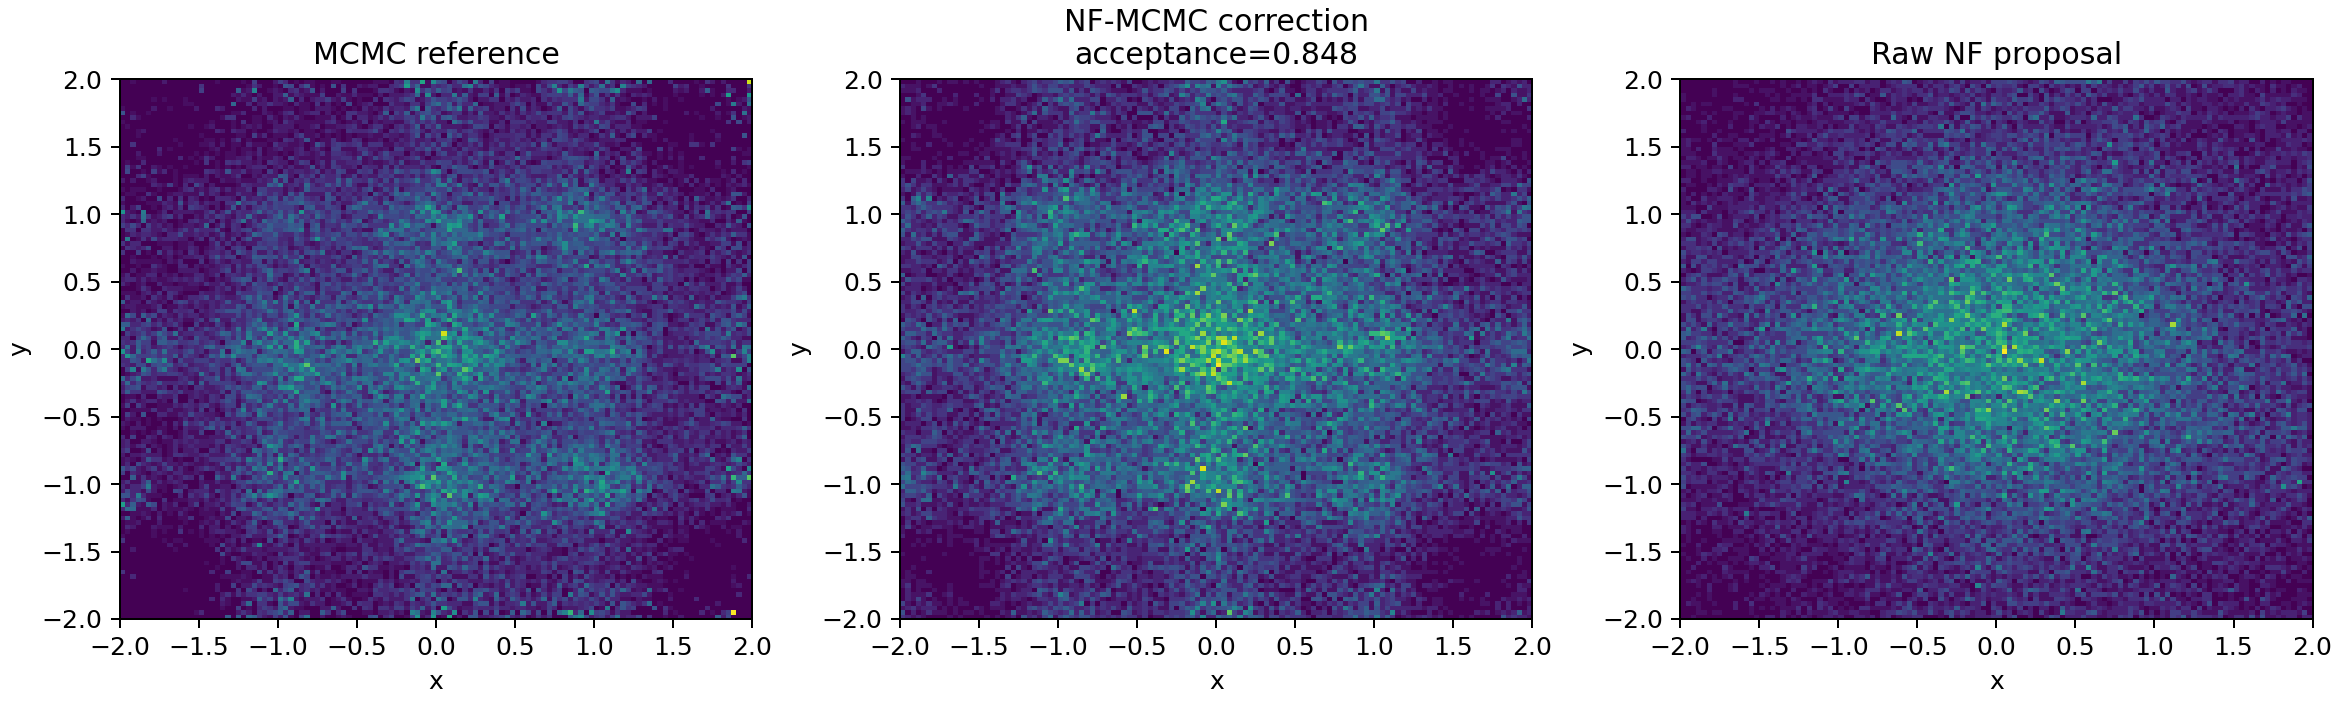
\includegraphics[width=\linewidth]{figures/ackley_nf_mcmc_correction.png}
  \caption{Two-dimensional Ackley diagnostic. The left panel is a random-walk MCMC reference, the center panel contains normalizing-flow proposals after MCMC correction, and the right panel contains raw normalizing-flow proposals. The acceptance value displayed inside the source figure is run-specific and should be replaced by a repeated-run summary in the final version.}
  \label{fig:ackley-nf-correction}
\end{figure}

\subsection{TMD event-level sampler diagnostics}
Figure~\ref{fig:tmd-marginals} compares event marginals from the real event batch with samples generated by inverse transform sampling (ITS) and the MCMC-corrected LOITS sampler. Figure~\ref{fig:tmd-xqt} shows the corresponding $x$--$q_T$ projection. These plots are application-level diagnostics and should be accompanied by the saved histogram metrics and the MCMC acceptance rate.

\begin{figure}[ht]
  \centering
  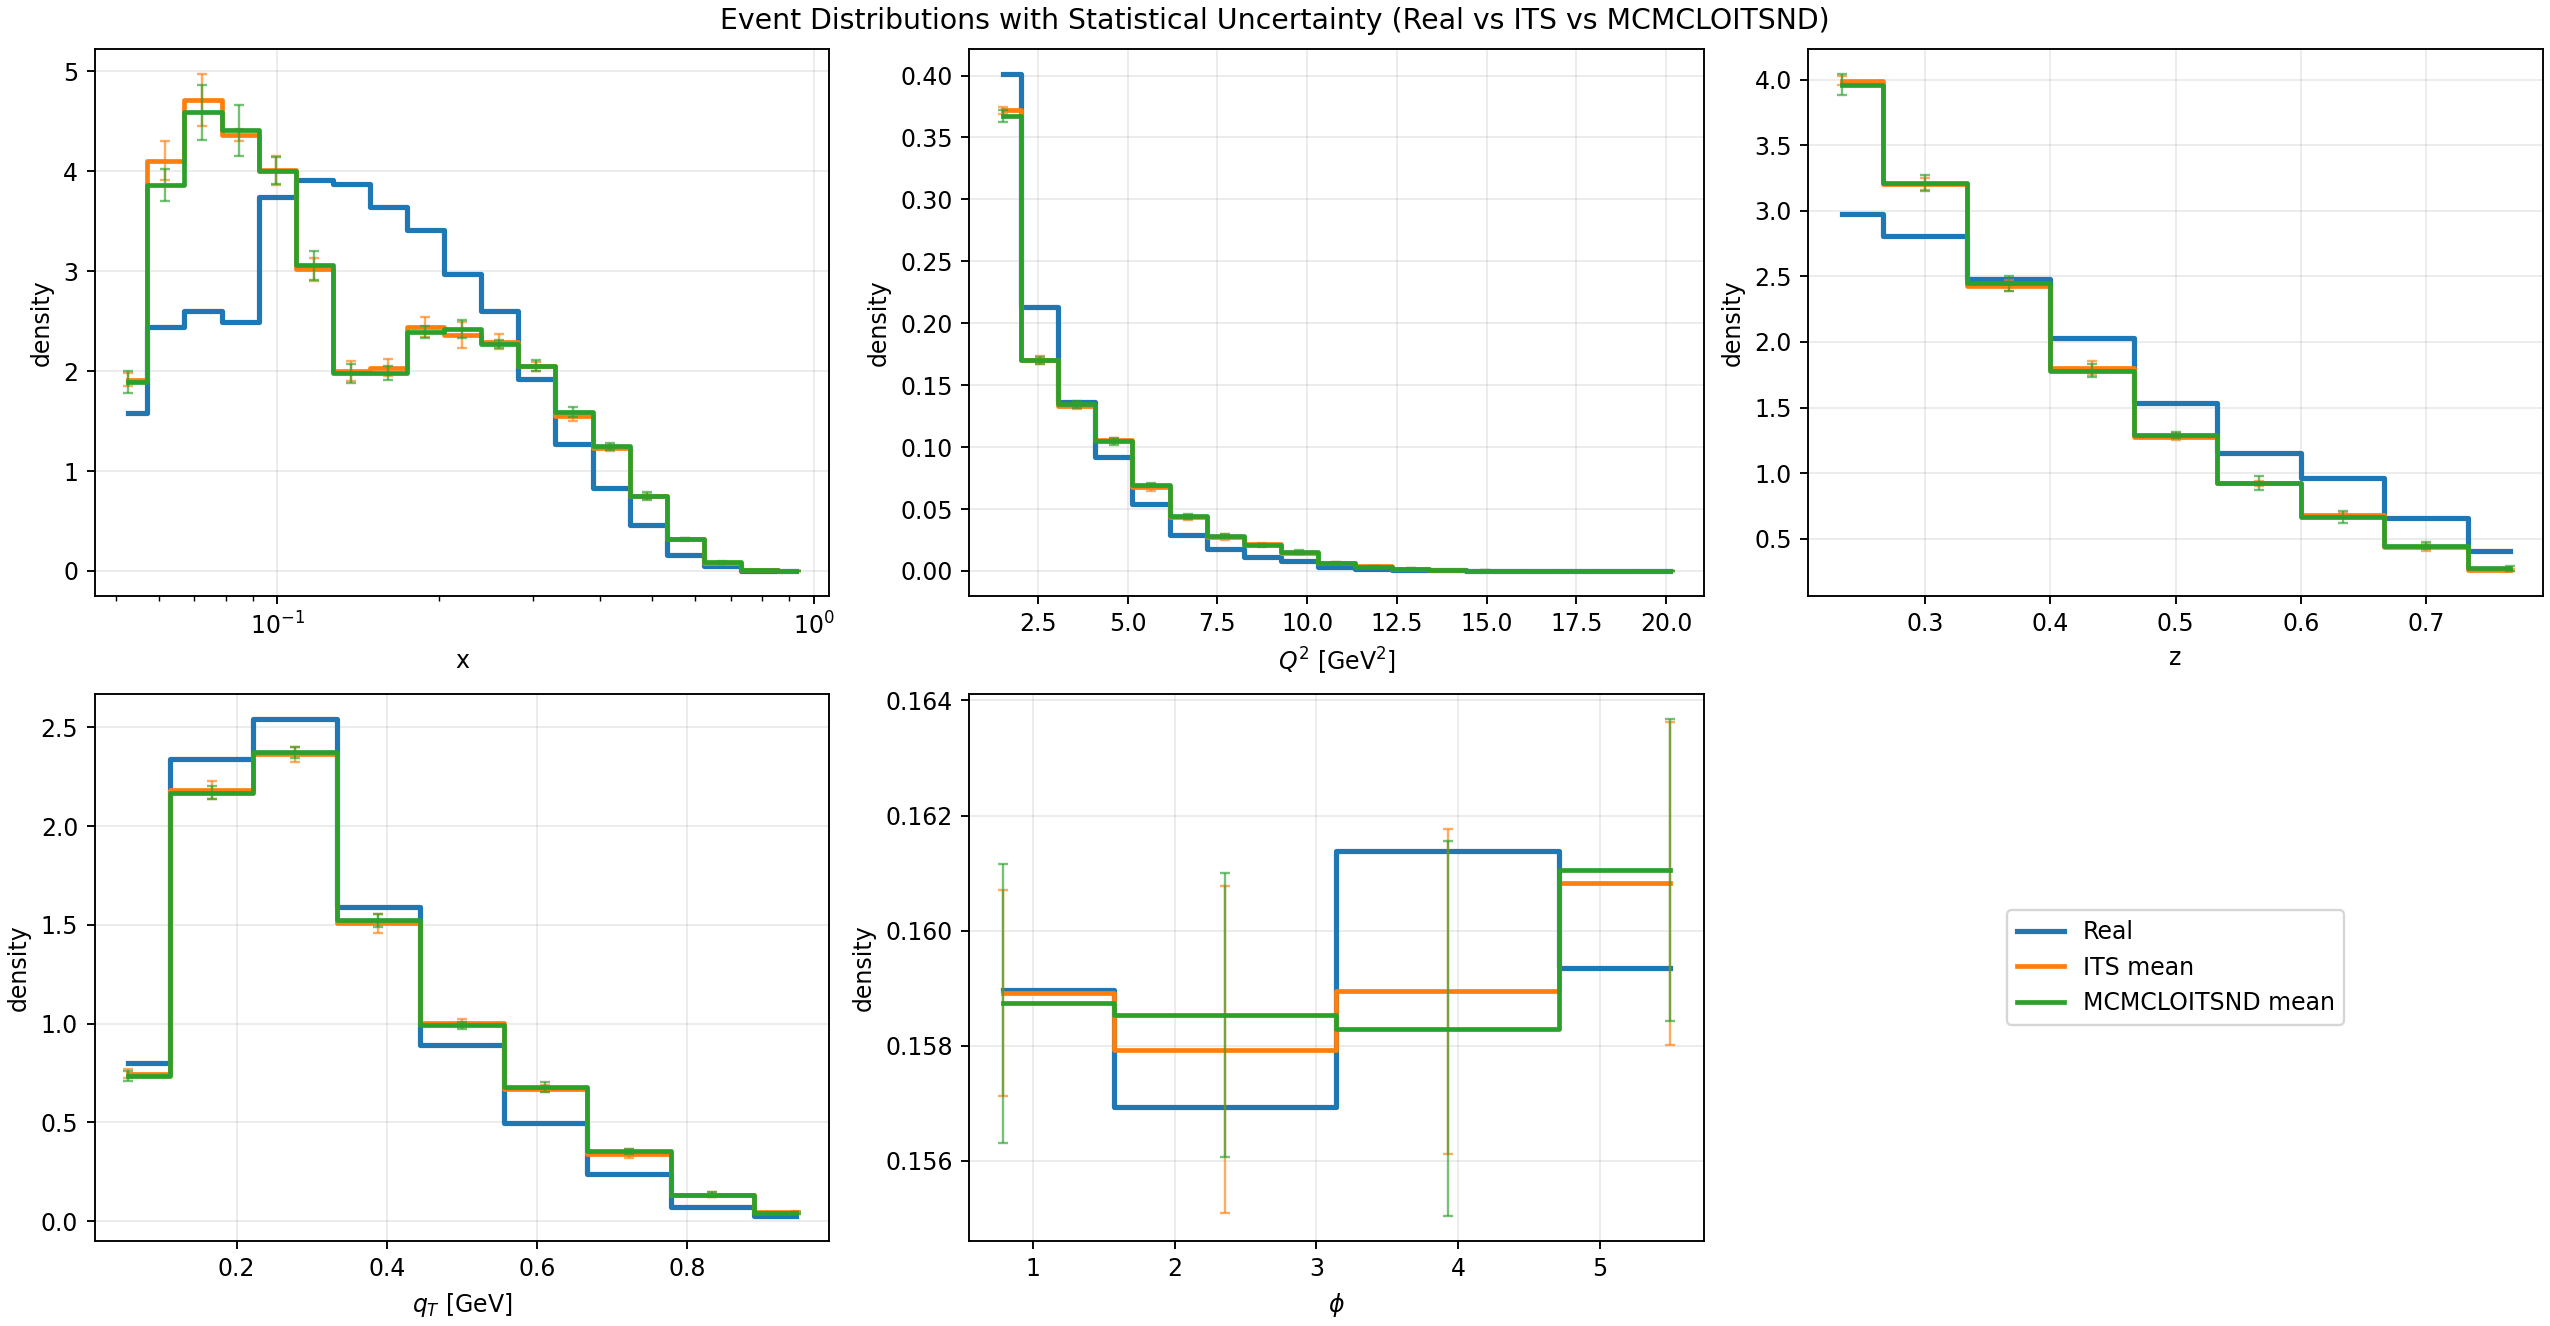
\includegraphics[width=\linewidth]{figures/tmd_event_marginals_its_mcmc_loits.png}
  \caption{TMD event marginal distributions. Blue denotes the real event batch; orange denotes the ITS sample mean; green denotes the MCMCLOITSND sample mean. Error bars summarize the sampling variation shown in the source experiment.}
  \label{fig:tmd-marginals}
\end{figure}

\begin{figure}[ht]
  \centering
  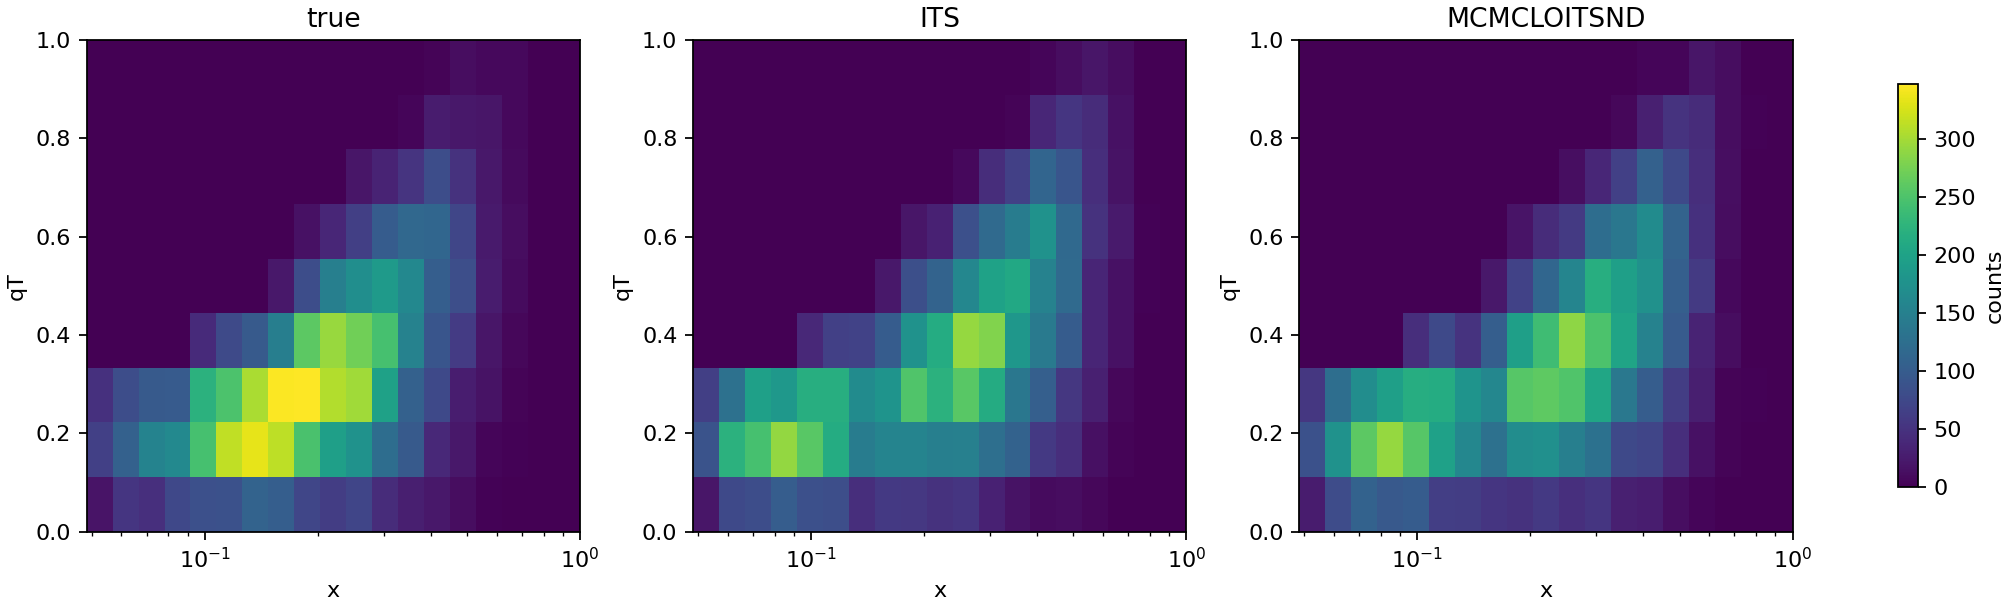
\includegraphics[width=\linewidth]{figures/tmd_x_qt_projection_its_mcmc_loits.png}
  \caption{TMD $x$--$q_T$ projection for the real event batch, ITS, and MCMCLOITSND. All panels use the same displayed binning; the colorbar reports counts.}
  \label{fig:tmd-xqt}
\end{figure}

\subsection{Acceptance rate versus dimension}
\todo{Jitao: insert the final LOITS-MCMC versus NF-MCMC curve only after the proposal definitions, training budgets, and repeated-run protocol are fixed. Explain the observed trend without claiming that acceptance alone establishes superior sampling quality.}

\begin{figure}[ht]
  \centering
  \fbox{\parbox{0.88\linewidth}{\centering
    \vspace{1.25in}
    \todo{Insert LOITS-MCMC and NF-MCMC acceptance rate versus dimensionality.}
    \vspace{1.25in}}}
  \caption{Placeholder for the dimensional acceptance comparison.}
  \label{fig:acceptance}
\end{figure}

\begin{table}[ht]
  \centering
  \caption{Placeholder for the numerical comparison. Values must be aggregated across repeated runs.}
  \label{tab:metrics}
  \begin{tabular}{lrrrr}
    \toprule
    Method & Acceptance & JS divergence & $L^1$ error & Density MAE \\
    \midrule
    \methodloits-MCMC & \todo{ } & \todo{ } & \todo{ } & \todo{ } \\
    \methodnf-MCMC & \todo{ } & \todo{ } & \todo{ } & \todo{ } \\
    \bottomrule
  \end{tabular}
\end{table}

\section{Discussion}
\label{sec:discussion}
The comparison separates two questions: whether a proposal is close enough to the target to attain a useful MCMC acceptance rate, and whether the corrected samples reproduce the target distribution at the desired resolution. A learned flow can improve a proposal when its training data and training budget are adequate. A grid-local inverse-transform proposal may be attractive when it requires no learned model, but its approximation quality can degrade in high dimension.

\todo{Joint: reconcile the final empirical trend with the theoretical discussion. Explicitly state limits arising from grid resolution, target choice, finite training data, and finite MCMC transitions.}

\section{Conclusion}
\todo{Joint: give a short conclusion after finalizing experimental results.}

\section*{Data and Code Availability}
The implementation and scripts used for the experiments will be released at \todo{repository URL or archival DOI}.

\section*{Acknowledgments}
\todo{Add funding, institutional support, and collaborator acknowledgments.}

\bibliographystyle{plainnat}
\bibliography{references}

\end{document}
